% chktex-file 44

\documentclass[a4paper,12pt]{article}
\usepackage[utf8]{inputenc}
\usepackage[russian]{babel}
\usepackage{geometry}
\usepackage{amsthm}
\usepackage[dvipsnames]{xcolor}
\usepackage{framed}
\usepackage{booktabs}
\usepackage{array}
\usepackage{amssymb}
\usepackage{adjustbox}
\usepackage{makecell}
\usepackage{float}
\usepackage{graphicx}

\definecolor{shadecolor}{RGB}{245,245,247} 
\geometry{left=2cm, right=2cm, top=2cm, bottom=2cm}

\title{Типовой расчет №1 \\ по математической статистике. \\ Часть I}
\author{Ким В.Р. \\ Группа M3207 \\ Вариант №5}
\date{}

\theoremstyle{definition}
\newtheorem{problem}{Задача}\setlength{\parindent}{0pt}

\newenvironment{solution}
{\begin{shaded}\textbf{Решение:}\par\setlength{\parindent}{0pt}}
{\end{shaded}}

\newenvironment{answer}
{\par\noindent\textbf{Ответ:} }
{\par}

\begin{document}

\maketitle

\par\noindent\textbf{Выборка \textit{(100 элементов)} :}
5.13 11.95 13.60 12.27 16.62 15.37 17.00 17.06 14.20 17.76 16.31 14.51 12.81 13.21 12.58
11.54 15.92 14.11 11.00 15.96 14.91 15.75 15.31 13.46 15.46 14.68 15.70 16.86 13.96 14.28
13.83 13.56 13.01 15.64 16.43 14.28 13.91 16.41 14.18 16.59 13.00 13.57 12.10 15.82 16.37
16.29 14.13 13.66 12.95 17.08 15.73 14.02 15.63 16.58 14.85 12.50 15.16 14.94 14.36 12.46
14.52 15.31 15.97 16.00 13.44 16.80 13.83 14.67 17.37 15.40 14.85 17.24 17.27 15.06 13.15
15.03 14.74 15.64 16.09 13.28 17.81 17.28 18.20 14.61 13.75 14.03 14.25 14.67 14.09 14.29
12.00 9.97 14.48 13.23 17.88 19.89 16.38 14.70 13.97 15.25
\\
\par\noindent\textbf{Отсортированная:}
5.13 9.97 11.00 11.54 11.95 12.00 12.10 12.27 12.46 12.50 12.58 12.81 12.95 13.00 13.01
13.15 13.21 13.23 13.28 13.44 13.46 13.56 13.57 13.60 13.66 13.75 13.83 13.83 13.91 13.96
13.97 14.02 14.03 14.09 14.11 14.13 14.18 14.20 14.25 14.28 14.28 14.29 14.36 14.48 14.51
14.52 14.61 14.67 14.67 14.68 14.70 14.74 14.85 14.85 14.91 14.94 15.03 15.06 15.16 15.25
15.31 15.31 15.37 15.40 15.46 15.63 15.64 15.64 15.70 15.73 15.75 15.82 15.92 15.96 15.97
16.00 16.09 16.29 16.31 16.37 16.38 16.41 16.43 16.58 16.59 16.62 16.80 16.86 17.00 17.06
17.08 17.24 17.27 17.28 17.37 17.76 17.81 17.88 18.20 19.89



\vspace{8pt}
% Задача 1
\begin{problem}
    Представить выборку из n=100 значений в виде вариационного ряда. Найти
    размах ряда $R = X_{max} - X_{min}$
        \begin{solution}
            \( R = 19.89 - 5.13 \approx 14.76\)
        \end{solution}

        \begin{answer}
            14.76
        \end{answer}

    \end{problem}



% Задача 2
\vspace{8pt}
\begin{problem}
    Построить интервальный статистический ряд, используя требуемое количество
    интервалов m (формула Стерженса) и вычислив ширину интервала \(h = R/m\)
    
        \begin{solution}
            Число интервалов по формуле Стёрженса: \( m = \log_2 (N) + 1 =7\) \\
            Ширина интервала: \( h = R/m = 14.76/7 \approx 2.109\) \\
            Интервальный статистический ряд - это столбцы "границы интервала" 
            и "частота" в следующем задании
        \end{solution}
    
        \begin{answer}
            7 интервалов, шириной 2.109
        \end{answer}
    
    \end{problem}



% Задача 3
\vspace{8pt}
\begin{problem}
    Результаты группировки свести в таблицу:

    \begin{table}[H]
        \centering
        \begin{adjustbox}{max width=\textwidth}
            \begin{tabular}{l c c c c c c c}
                \toprule
                    \makecell{Номер\\интервала \( i \)} & 
                    \makecell{Границы \\ интервала \( i \)} & 
                    \makecell{Середина\\интервала \( x_i \)} & 
                    \makecell{Частота\\\( n_i \)} & 
                    \makecell{Отн. частота\\\( W_i = \frac{n_i}{N} \)} & 
                    \makecell{Накопл.\\частота\\\( \sum^i_j n_i \)} & 
                    \makecell{Накопл. отн.\\частота\\\( \sum^i_j \frac{n_i}{N} \)} & 
                    \makecell{Плотность\\отн. частоты\\\( \frac{W_i}{h} \)} \\
                        \midrule
                            \dots & \dots & \dots & \dots & \dots & \dots & \dots & \dots \\
                        \bottomrule
            \end{tabular}
        \end{adjustbox}
    \end{table}  

    \begin{solution}
        \begin{table}[H]
            \centering
            \begin{adjustbox}{max width=\textwidth}
                \begin{tabular}{l c c c c c c c}
                    \toprule
                        \makecell{Номер\\интервала \( i \)} & 
                        \makecell{Границы \\ интервала \( i \)} & 
                        \makecell{Середина\\интервала \( x_i \)} & 
                        \makecell{Частота\\\( n_i \)} & 
                        \makecell{Отн. частота\\\( W_i = \frac{n_i}{N} \)} & 
                        \makecell{Накопл.\\частота\\\( \sum^i_j n_i \)} & 
                        \makecell{Накопл. отн.\\частота\\\( \sum^i_j \frac{n_i}{N} \)} & 
                        \makecell{Плотность\\отн. частоты\\\( \frac{W_i}{h} \)} \\
                            \midrule
                                1 & [5.13; 7.24) & 6.18 & 1 & 0.01 & 1 & 0.01 & 0.0047 \\
                                2 & [7.24; 9.35) & 8.29 & 0 & 0 & 1 & 0.01 & 0 \\
                                3 & [9.35; 11.46) & 10.40 & 2 & 0.02 & 3 & 0.03 & 0.0095 \\
                                4 & [11.46; 13.56) & 12.51 & 19 & 0.19 & 22 & 0.22 & 0.0901 \\
                                5 & [13.56; 15.67) & 14.62 & 46 & 0.46 & 68 & 0.68 & 0.2182 \\
                                6 & [15.67; 17.78) & 16.73 & 28 & 0.28 & 96 & 0.96 & 0.1328 \\
                                7 & [17.78; 19.89) & 18.84 & 4 & 0.04 & 100 & 1 & 0.019 \\
                            \bottomrule
                \end{tabular}
            \end{adjustbox}
        \end{table}  
    \end{solution}
    \end{problem}



% Задача 4
\vspace{8pt}
\begin{problem}
    По результатам группировки построить 
    \begin{itemize}
        \item Полигон абсолютных частот (ломаная с вершинами в точках \((x_i; n_i)\)
        \item Гистограмму относительных частот
        \begin{itemize}
            \item и на ней полигон относительных частот, соединив отрезками прямой 
            середины верхних сторон прямоугольников гистограммы.
        \end{itemize}
        \item Гистограмму плотностей относительных частот(ступенчатую фигуру
        из прямоугольников с основаниями, равными интервалам значений признака, и
        высотами, равными частостям/плотностям частостей интервалов)
    \end{itemize}
    
        \begin{solution}
            \begin{figure}[H]
                \centering
                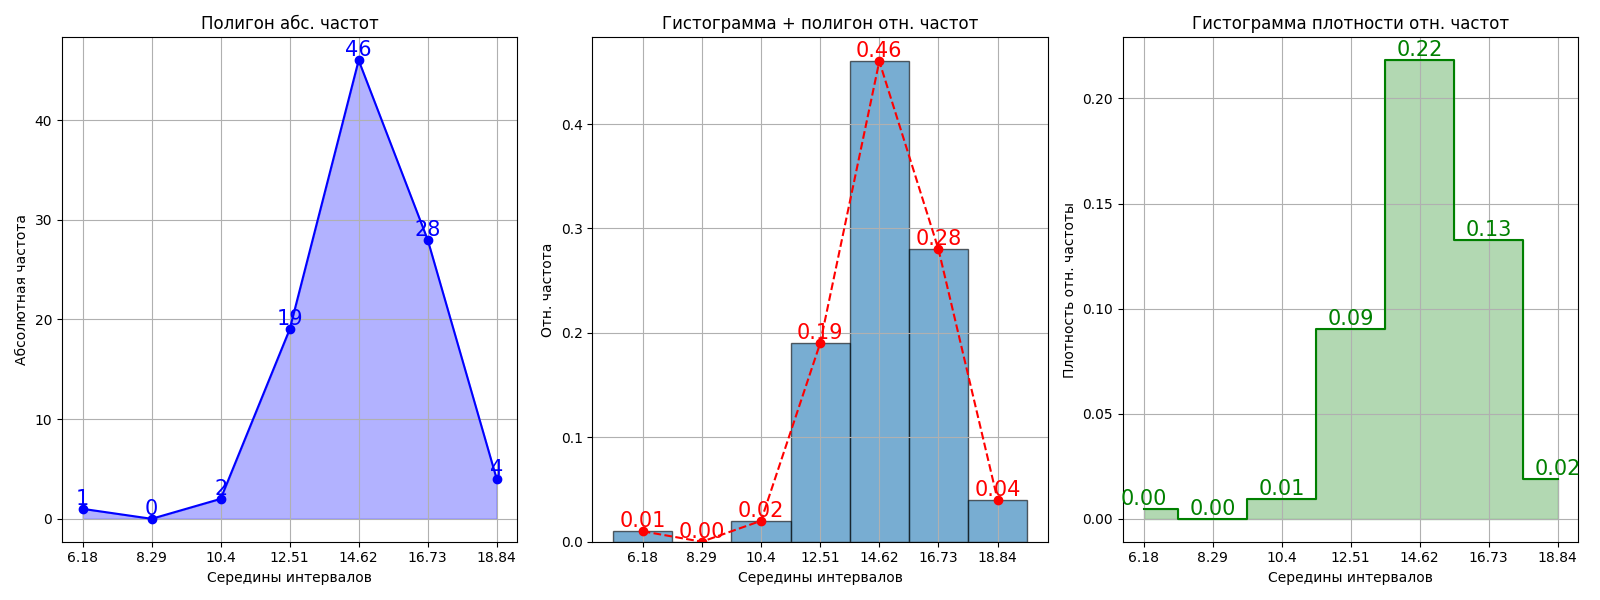
\includegraphics[width=1\textwidth]{plots/1.1.4.png}
            \end{figure}
            
        \end{solution}
    
        % \begin{answer}
            
        % \end{answer}
    
    \end{problem}



% Задача 5
\vspace{8pt}
\begin{problem}
    Построить эмпирическую функцию распределения интервального ряда \(F_n(x)\)), то
    есть относительную частоту (частость) того, что признак (случайная величина \(X\)) 
    примет значение, меньшее заданного \(x\) , т.е. \(F_n(x) = w(X < x)\) . 
    Для данного \(х\) эмпирическая функция распределения представляет 
    накопленную частость \(w^{acc}_x = \frac{n^{acc}_x}{n}\).
    Графиком эмпирической функции распределения является кумулята накопленных
    относительных частот, то есть ломаная, вершины которой имеют абсциссы,
    совпадающие с правыми границами интервалов группировки, и ординаты,
    совпадающие со значениями накопленных частот для соответствующих
    интервалов.
    
        \begin{solution}
            \begin{figure}[H]
                \centering
                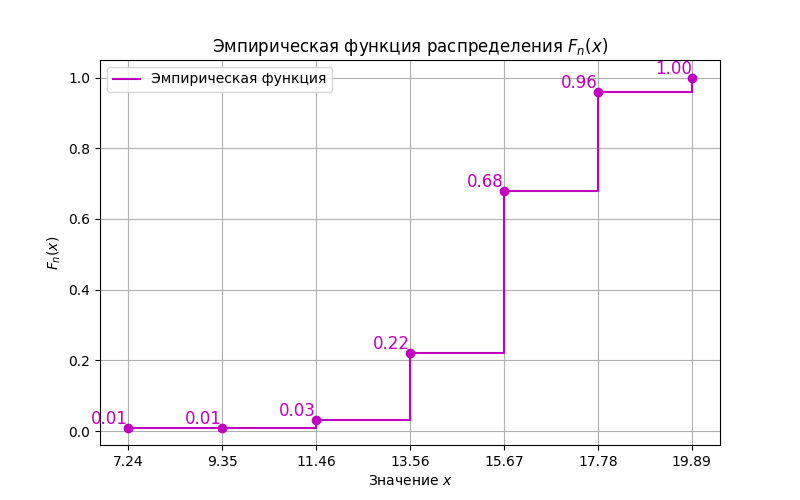
\includegraphics[width=0.8\textwidth]{plots/1.1.5.png}  
            \end{figure}
        \end{solution}
    
        % \begin{answer}
        % \end{answer}
    
    \end{problem}


% Задача 6
\vspace{8pt}
\begin{problem}
    Найти эмпирическую функцию распределения дискретного вариационного ряда
    (cередины интервалов – накопленные относительные частоты).
    Здесь эмпирическая функция распределения представляет собой разрывную
    ступенчатую функцию по аналогии с функцией распределения для дискретной
    случайной величины с той разницей, что по оси ординат вместо вероятностей –
    накопленные частости
    
        \begin{solution}
            \begin{solution}
                \begin{figure}[H]
                    \centering
                    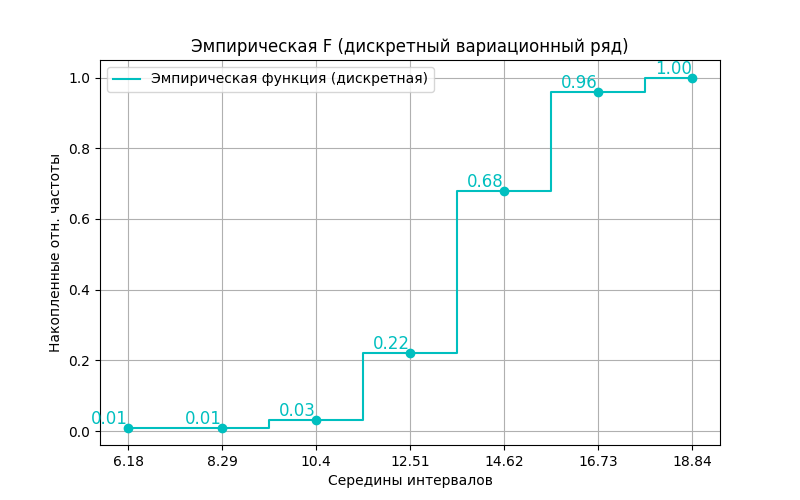
\includegraphics[width=0.8\textwidth]{plots/1.1.6.png}  
                \end{figure}
            \end{solution}
        \end{solution}
    
        % \begin{answer}
        % \end{answer}
    
    \end{problem}



% Задача 7
\vspace{8pt}
\begin{problem}
    Найти оценки математического ожидания (выборочное среднее), несмещенную и
    смещенную оценки дисперсии и среднего квадратического отклонения.
    
        \begin{solution}
            Выборочное среднее 
            \[ \bar{x} = \sum^m_{i=1} x_i w_i = 14.81,\] 
            где \(w_i\) - это отн. частота \(i\) \\

            Смещенная оценка дисперсии 
            \[ s^2 = \sum^m_{i=1}(x_i - \bar{x})^2 w_i = 3.84 \] \\

            Несмещенная оценка дисперсии 
            \[ \hat{s^2} = \frac{n}{n-1} s^2 = 3.88 \] \\

            Среднеквадратичное отклонение = \[ s = \sqrt{s^2} = 1.97 \]
        \end{solution}
    
        \begin{answer}
        \end{answer}
    
    \end{problem}



% Задача 8
\vspace{8pt}
\begin{problem}
    Найти медиану вариационного ряда \(\hat{M_e}\) ( значение признака, приходящегося на
    середину вариационного ряда). Для интервального вариационного ряда медиана
    находится с помощью линейного интерполирования медианного интервала ряда
    или с помощью кумуляты накопленных частот, как значение признака, для
    которого накопленная частота равна \(0.5\)
    
        \begin{solution}
            Для вариационного ряда с \( n = 100 \), значение посередине равно среднему между значениями 
            под номерами 50 и 51:
            \[ \hat{M_e} = (14.68 + 14.7) / 2 = 14.69\]

            Решение для интервального вариационного ряда:\\
            \(n/2 = 100/2 = 50.\)\\
            Медианным интервалом \([L_m, U_m]\) является интервал, в котором лежит накопленная частота,
            равная либо наименьшая превышающая 50, то есть, интервал \([13.56; 15.67)\)
            с частотой \(f_m = 46\)\\
            Кумулятивная частота \(F_{m-1}\) интервала предшествующего медианному равна \(19\)
            Ширина интервалов \(h\) равна 2.109 \\


            \[ \hat{M_e} = L_m + \frac{h(\frac{n}{2} - F_{m-1})}{f_m} \]
            \[ \hat{M_e} = 13.56 + \frac{2.109(50 - 19)}{46} \approx 14.98\]
            
        \end{solution}
    
        \begin{answer}
            14.98
        \end{answer}
    
    \end{problem}



% Задача 9
\vspace{8pt}
\begin{problem}
    Найти моду вариационного ряда \(\hat{M_o}\) (вариант, которому соответствует
    наибольшая частота). Для интервального ряда значение моды определяется с
    помощью линейного интерполирования модального интервала
    
        \begin{solution}
            Для вариционного ряда: максимальная частота в выборке равна 2, ее имеют элементы
            13.83, 14.28, 14.67, 14.85, 15.31, 15.64.  \\

            Решение для интервального вариационного ряда: \\
            модальный интервал \([L_m; U_m]\) (или интервал с наибольшей частотой) - \( [13.56; 15.67) \). \\
            Его частота \(f_m\) равна 46. \\
            Частота интервала до него \(f_{m-1}\) равна 19, после (\(f_{m+1}\)) - 28 (из задачи №3).\\
            Ширина интервалов \(h\) равна 2.109 \\
            Тогда по методу линейного интерполирования модального интервала, мода \(\hat M_e\) вычисляется по формуле:
            \[ \hat{M_o} = L_m + \frac{h(f_m - f_{m-1})}{2(f_m - f_{m-1}) + (f_m - f_{m+1})}, \]
            \[ \hat{M_o} = 13.56 + \frac{2.109(46 - 19)}{2(46 - 19) + (46 - 28)} \approx 14.35\]
        \end{solution}
    
        \begin{answer}
            14.35
        \end{answer}
    
    \end{problem}



% Задача 10
\vspace{8pt}
\begin{problem}
    Вычислить коэффициент ассиметрии вариационного ряда
    \[\tilde{A} = \frac{\tilde{\mu_3}}{s^3},\]
    \[\tilde{\mu_k} = \frac{\sum^m_{i=1}(x_i - \bar{x})^k n_i}{n},\] 
    где \(m\) - число неповторяющихся вариантов или число интервалов     
        
    \begin{solution}
        \(s = 1.97\), \( s^3 = 1.97^3 \approx 7.65 \)\\
        \(\bar{x} = 14.81\) (из задания 7)\\

        Вычислим третий момент:
        \[ \tilde{\mu_3} = \frac{\sum^m_{i=1}(x_i - \bar{x})^3 n_i}{n} = 
        \frac{(      -642.71\cdot1 
                     -85.76\cdot2 
                     -12.17\cdot19
                     -0.01\cdot46
                     +7.08\cdot28
                     +65.46\cdot4
                     )}{100} \]
            \[ \approx \frac{-585.84}{100} \approx -5.86 \]
        \(\hat{\mu_3} < 0\) говорит о левосторонней ассиметрии. \\
        
        Тепепрь считаем коэффициент ассиметрии:
        \[ \tilde{A} = \frac{\tilde{\mu_3}}{s^3} = \frac{-5.86}{7.65} \approx - 0.77\]

        \end{solution}
    
        \begin{answer}
            -0.77
        \end{answer}
    
    \end{problem}



% Задача 11
\vspace{8pt}
\begin{problem}
    Вычислить коэффициент эксцесса вариационного ряда
    \[\tilde{E} = \frac{\tilde{\mu_4}}{s^4} - 3\]
    
        \begin{solution}
            \(s = 1.97\), \( s^4 = 1.97^4 \approx 15.06 \)\\
        \(\bar{x} = 14.81\) (из задания 7)\\

        Вычислим четвертый момент:
        \[ \tilde{\mu_3} = \frac{\sum^m_{i=1}(x_i - \bar{x})^3 n_i}{n} = 
        \frac{(     5547\cdot1
                    378\cdot2
                    28\cdot19
                    14\cdot28
                    264\cdot4
                     )}{100} \]
            \[ \approx \frac{8270.23}{100} \approx 82.7 \]
        \(\hat{\mu_4} > 0\) говорит о сосредоточенности значений вокруг среднего 
        (заостренная вершина графика по сравнению с нормальным распределением). \\
        
        Тепепрь считаем коэффициент эксцесса:
        \[ \tilde{A} = \frac{\tilde{\mu_4}}{s^4} = \frac{82.7}{15.06} \approx 5.49\]

        \end{solution}
    
        \begin{answer}
            5.49
        \end{answer}
    
    \end{problem}

\end{document}